\subsection{Formulasi Masalah}
\label{subsec:traffic-forecasting-problem-formulation}
Diberikan sekuens data pengamatan lalu lintas sejumlah $M$ \textit{time steps} $\textbf{X}=\{x_{t-M+1},x_{t-M+2},\ldots,x_{t} \}, \ x_t\in \mathbb{R}^N$. $x_t$ adalah vektor kecepatan dari sejumlah $N$ segmen jalan pada waktu $t$. Tujuan prediksi kecepatan lalu lintas adalah memprediksi sekuens nilai dari $Y=\{x_{t+1},x_{t+2},\ldots,x_{t+Q}\}$. Graf jaringan jalan $G=(V,E)$ terdiri dari himpunan simpul $V$ yang berjumlah $N$ simpul  dan himpunan sisi $E$. Misalkan $v\in V$ adalah simpul dan $e=(v,u)\in E$ adalah sisi yang menghubungkan $v$ dengan $u$. $N(v)=\{u\in V\mid (v,u)\in E\}$ adalah tetangga dari simpul $v$. Matriks $adjacency$ $A\in \mathbb{R}^{N\times N}$ adalah representasi matematis dari graf, dengan $A_{ij}=c>0$ jika $(v_i,v_j)\in E$ dan $A_{ij}=0$ jika $(v_i,v_j)\notin E$. Simpul adalah stasiun pemantau lalu lintas dan sisi menunjukkan keterhubungan antar stasiun.

\subsection{Arsitektur Multivariate Time-Series Graph Neural Network (MTGNN)}
\label{subsec:traffic-forecasting-mtgnn-architecture}
Arsitektur dari MTGNN terdiri dari, \textit{graph learning layer}, sejumlah $m$ \textit{graph convolution layer}, sejumlah $m$ \textit{temporal convolution layer}, dan sebuah \textit{output layer} (\cite{Wu2020}). \textit{Graph learning layer} mempelajari matriks \textit{adjacency} graf secara adaptif untuk menangkap hubungan tersembunyi di antara data \textit{traffic time series} tanpa perlu menentukan struktur graf secara eksplisit (\cite{Wu2020}). \textit{Graph learning layer} didefinisikan dengan:

\begin{align}
    \mathbf{M}_1 &= \tanh(\alpha \mathbf{E}_1 \mathbf{\Theta_1})\\
    \mathbf{M}_2 &= \tanh(\alpha \mathbf{E}_1 \mathbf{\Theta_1})\\
    \mathbf{A} &= \mathrm{ReLU}\bigl(\tanh\bigl(\alpha(\mathbf{M}_1\mathbf{M}_2^{T}-\mathbf{M}_2\mathbf{M}_1^{T})\bigr)\bigr) \\ 
    i \; &= \; 1,2,\ldots,N \\
   \hspace{2em}  \mathbf{idx} &= \mathrm{argtopk}(\mathbf{A}[i,:])\\
     \mathbf{A}[i,-\mathbf{idx}] &= 0, 
\end{align}

Dimana $\mathbf{E}_1,\mathbf{E}_2\in \mathbb{R}^{N\times d_e}$ adalah \textit{node embeddings} yang dinisialisasi secara acak dan dapat dipelajari selama pelatihan. $\mathbf{\Theta_1},\mathbf{\Theta_2}\in \mathbb{R}^{d_e \times d_t}$ adalah parameter model, dan $\alpha$ adalah \textit{hyperparameter} untuk mengontrol tingkat saturasi dari fungsi aktivasi, dan $argtopk(\cdot)$ mengembalikan indeks dari sejumlah k nilai terbesar dari vektor.\textit{ Graf learning layer} mengekstrak hubungan \textit{uni-directional} dari setiap simpul. Hal ini disebabkan karena ketika $A_{vu}>0$, maka nilai sisi terbaliknya $A_{uv}=0$. 
\begin{align}
    T_{uv}=tanh(\alpha(M_{1u}M_{2v}^T-M_{2u}M_{1v}^T))\\
    T_{vu}=tanh(\alpha(M_{1v}M_{2u}^T-M_{2v}M_{1u}^T))\\
    T_{vu}=-T_{uv}\\
    A_{vu}=Relu(-T_{uv})=\max (0,-T_{uv})=0
\end{align}

Persamaan (3.19)-(3.20) membuat matriks $adjacency$ graf menjadi \textit{sparse} dengan cara menetapkan nilai $adjacency$ tetangga-tetangga yang tidak terlalu relevan (tidak termasuk \textit{top} k nilai terbesar dari vektor $\mathbf{A[i,:]}$) dari setiap simpul $i$ sama dengan nol.

\textit{Graph Convolution layer} mempelajari ketergantungan spasial menggunakan dua \textit{mix-hop }\textit{propagation layers} untuk memproses informasi aliran lalu lintas masuk dan keluar yang melewati setiap simpul secara terpisah. Gambar~\ref{fig:gc-layer} menunjukkan arsitktur dari \textit{graph convolution layer}. \textit{Mix-hop propagation layer} dapat mempelajari kombinasi linear fitur-fitur dari simpul-simpul tetangga yang memiliki jarak beberapa \textit{hop} dari suatu simpul. \textit{Mix-hop propagation layer} terdiri dari tahapan \textit{information propagation} dan tahapan \textit{information selection}. Tahapan \textit{information propagation} menyebarkan informasi simpul-simpul mengikuti struktur graf yang sudah dipelajari. Arsiktektur mix-hop propagation layer ditampilkan pada Gambar~\ref{fig:mixhop-layer}. Tahapan \textit{information propagation} didefinisikan dengan:
\begin{equation}
    \mathbf{H}^{(k)}=\beta \mathbf{H}_{in}+(1-\beta ) \tilde{\mathbf{A}} \mathbf{H}_{(k-1)}
\end{equation}


\begin{figure}[H]
    \centering
    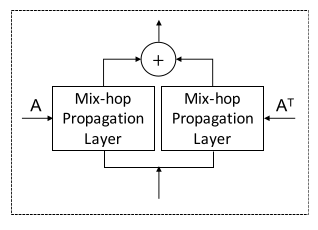
\includegraphics[]{figures/gc_layer.png}
    \caption{Arsitektur dari Graph Convolution Layer (diadaptasi dari~\cite{Wu2020})}
    \label{fig:gc-layer}
\end{figure}



\begin{figure}[H]
    \centering
    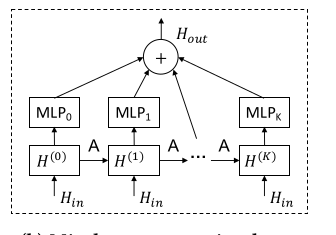
\includegraphics[]{figures/mix_hop.png}
    \caption{Arsitektur dari Mix-hop Propagation Layer (diadaptasi dari~\cite{Wu2020})}
    \label{fig:mixhop-layer}
\end{figure}


Dimana $\beta$ adalah \textit{hyperparameter} yang mengatur rasio antara fitur \textit{hidden states}  pada \textit{layer} sebelumnya dengan informasi \textit{hidden states} pada \textit{hop} sebelumnya $(k-1)$ yang akan dipertahankan pada \textit{hidden states} pada \textit{hop} $k$. Tahapan \textit{information selection} menggabungkan berbagai fitur \textit{hidden states} pada setiap \textit{hop} dengan memberikan bobot $\mathbf{W}^{k}$ pada setiap fitur. Tahapan \textit{information selection} didefinisikan dengan:
\begin{equation}
    \mathbf{H}_{out} = \sum_{i=0}^{K}\mathbf{H}^{(k)}\mathbf{W}^{(k)}
\end{equation}

Temporal Convolution Layer mengekstrak  fitur temporal dari data \textit{time series} lalu lintas melalui serangkaian operasi \textit{1D convolutional filters}. Arsitektur dari temporal Convolutional layer ditunjukkan pada Gambar~\ref{fig:tc-layer}. Temporal Convolution Layer terdiri dari dua \textit{dilated inception layers}. Kedua \textit{dilated inception layer} tersebut menjadi input dari Gated Linear Unit (GLU) dengan satu input memiliki fungsi aktivasi tangen hiperbolik dan satunya lagi memiliki fungsi aktivasi \textit{sigmoid}. GLU berfungsi sebagai gerbang yang mengontrol banyaknya informasi hasil dari \textit{dilated convolution} yang dapat diteruskan pada \textit{layer} selanjutnya. \textit{Dilated convolution layer} menjalankan beberapa \textit{dilated convolution} dengan setiap \textit{convolution} memliki ukuran kernel yang berbeda-beda. Hal ini membuat model dapat mempelajari pola temporal dari data dengan berbagai rentang waktu (\textit{short-term}, \textit{long-term}, dan \textit{medium-term}) dan membuat model mampu mengaproksimasi stuktur \textit{optimal network topology} (\cite{Wu2020}). \textit{Dilated convoluton layer} memberikan jarak pada setiap bobot \textit{convolution kernel} dan membuat ukuran \textit{reception field } dari model meningkat secara eksponensial. \textit{Dilated convolution layer} membuat model mampu menangkap pola sekuens yang lebih panjang. \textit{Dilated convolution operation} pada setiap kernel didefinisikan dengan:
\begin{equation}
    \mathbf{z} \star \mathbf{f}_{1\times k}(t)  =b+\sum_{j=0}^{k-1}  \mathbf{f_{1\times k}}[j] \mathbf{z}[t-d\times j]
\end{equation}

\textit{Dilated convolution layer} didefinisikan dengan:
\begin{equation}
    z_{out}= concat(\mathbf{z} \star \mathbf{f}_{1\times 2}(t), \mathbf{z} \star \mathbf{f}_{1\times 3}(t), \mathbf{z} \star \mathbf{f}_{1\times 6}(t), \mathbf{z} \star \mathbf{f}_{1\times 7}(t))
\end{equation}

\begin{figure}[H]
    \centering
    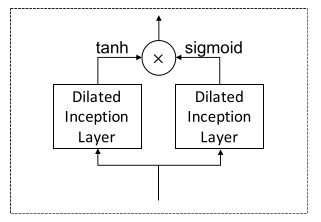
\includegraphics[]{figures/tc_layer.png}
    \caption{Arsitektur dari Temporal Convolution Layer (diadaptasi dari~\cite{Wu2020})}
    \label{fig:tc-layer}
\end{figure}

\cite{Wu2020} menambahkan \textit{Residual Connection Layer} yang meneruskan input dari Temporal Convolution layer ke output dari Graph Convolution Layer  dan mnambahkan \textit{skip connections} yang meneruskan output dari setiap Temporal Convolution Layer ke output layer. Hal ini bertujuan untuk mencegah terjadinya \textit{vanishing gradient problem} pada saat \textit{training} model. Output layer tediri dari dua 1x1 \textit{convolution layer} yang memetakan input ke dimensi output $Q$. Dimana $Q$ adalah jumlah \textit{step} prediksi yang diinginkan. Arsitektur dari Multivariate Time-Series Graph Neural Network ditunjukkan pada Gambar~\ref{fig:mtgnn-architecture}. MTGNN menggunakan \textit{L2 loss function}/\textit{mean squared error}  untuk mengukur performa dari model. MTGNN dilatih dengan menggunakan \textit{curriculum learning}, dimana algoritma dimulai dengan memprediksi satu \textit{time step}. Seiring bertambahnya iterasi, panjang prediksi model meningkat secara bertahap. \textit{Pseudocode} untuk  \textit{curiculum learning} ditunjukkan pada Algoritma~\ref{alg:mtgnn-learning}.


\begin{algorithm}
\caption{Curiculum Learning dengan input \textit{dataset} $O$, model $f(\cdot)$, parameter model $\Theta$, \textit{learning rate} $\gamma$, \textit{batch size} $b$, \textit{step size} $s$, \textit{split size} $m$}
\label{alg:mtgnn-learning}
\resizebox{\textwidth}{!}{%
\begin{minipage}{\textwidth}
\scriptsize
\begin{algorithmic}[1]
\setstretch{0.9}
    \Procedure{CuriculumLearning}{$O, f(\cdot), V, \Theta, \gamma,  b, s, m$}
        \State $iter\gets 1, r \gets 1$
        \While{$\textbf{until convergence}$}
            \State $\text{sampel satu batch }  \mathcal{X}\in \mathbb{R}^{b\times T \times N \times D}, \mathcal{Y}^{b\times T' \times N} \text{ dari } O $
            \State $\text{random split } V \text{ menjadi } m \text{ grup } \cup_{i=1}^{m}V_i=V$
            \If {$iter \% s=0 \text{ and }  r\leq T'$}
                \State $r \gets r+1$
            \EndIf
            \For {$i =1 \to m$}
                \State $\text{hitung }  \hat{\mathcal{Y}} \gets f(\mathcal{X}[:,:,id(V_i),:], \Theta)$
                \State $\text{hitung } L\gets MSE(\hat{\mathcal{Y}}[:,:r,:], \mathcal{Y}[:,:r,id(V_i)])$
                \State $\text{update parameter } \Theta \text{ berdasarkan \textit{gradient} dari \textit{loss function} dan \textit{learning rate }} \gamma$ 
            \EndFor 
            \State $iter \gets iter+1$
            \EndWhile 
    \EndProcedure
\end{algorithmic}
\end{minipage}%
}
\end{algorithm}

\begin{figure}[H]
    \centering
    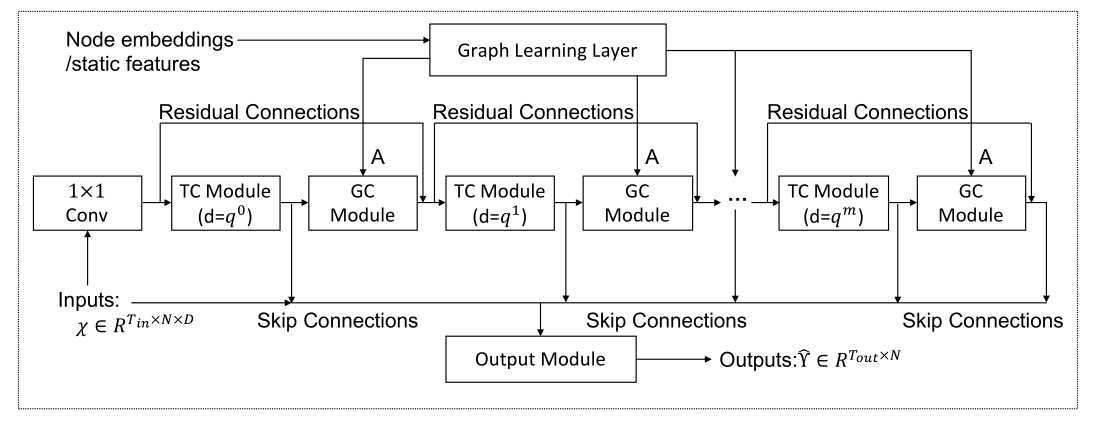
\includegraphics[width=0.9\textwidth]{figures/mtgnn.png}
    \caption{Arsitektur dari Multivariate Time-Series Graph Neural Network (diadaptasi dari~\cite{Wu2020})}
    \label{fig:mtgnn-architecture}
\end{figure}
